\documentclass[10pt,compress,t,notes=noshow, xcolor=table]{beamer}

\input{../../style/preamble}
\input{../../latex-math/basic-ml.tex}
\input{../../latex-math/basic-math.tex}

\usepackage{makecell}
% Defines macros and environments

\newcommand{\tab}[1][1cm]{\hspace*{#1}}

\definecolor{imllightblue}{RGB}{184, 198, 210}
\definecolor{imlmedblue}{RGB}{90, 122, 151}
\definecolor{imldarkblue}{RGB}{7, 55, 99}
\definecolor{imlhuegreen}{RGB}{0, 191, 196}
\definecolor{imlhuered}{RGB}{248, 118, 109}

\tikzset{main node/.style={rectangle,draw,minimum size=1cm,inner sep=4pt},}

\title{Interpretable Machine Learning}
% \author{LMU}
%\institute{\href{https://compstat-lmu.github.io/lecture_iml/}{compstat-lmu.github.io/lecture\_iml}}

\begin{document}

\titlemeta{
Intro to IML
}{
Dimensions of Interpretability
}{
figure/model_agnostic
}{
%\item What is interpretable machine learning (IML) and Explainable Artificial Intelligence (XAI)?
%: feature attribution vs. data attribution vs. counterfactual explanations
\item Difference between intrinsic, model-specific, and model-agnostic interpretability
\item Different types of explanations
\item Local, global, and regional explanations
\item Model/learner explanation (with(out) refits)
\item Levels of interpretability
}

%
% \begin{frame}{Interpretable ML}
% \begin{itemize}
% %\itemsep2em
% \item ML algorithms algorithmically train predictive models with no or little pre-specifications and assumptions about the data.
% \item Several algorithms such as decision tree learning create interpretable models. However, most algorithms create models which can be considered a black box.
% \item We use the term black box, although the internal workings of the model are in fact accessible, but too complex for the human mind to comprehend.
% \end{itemize}
% \end{frame}
%
% \begin{frame}{Explainable AI}
% \begin{itemize}
% %\itemsep1em
% \item IML is often used synonymously with Explainable AI (XAI).
% \item There is no unified standard for these terminologies. We find that XAI often is specifically concerned with the interpretation of neural networks, whereas IML is used as an encompassing term for everything related to model interpretability.
% \item The nature of (deep) neural networks allows for powerful model-specific interpretation techniques, e.g., layer-wise relevance propagation (LRP) and saliency maps.
% \item Also covering model-specific NN methods would exceed the timeframe of this lecture. This lecture will concentrate on model-agnostic techniques, as they are both versatile, and receive a lot of attention in industry and academia.
% \end{itemize}
% \end{frame}
%
% \begin{frame}{XAI - Saliency Maps}
%
% A saliency map is a heatmap indicating pixel influence on the prediction (e.g., a classification of an image): \footnote[frame]{Mundhenk, T., Chen, B.Y., Friedland, G. (2019). Efficient Saliency Maps for Explainable AI. ArXiv, abs/1911.11293.
% }
% \medskip
% \begin{figure}
% 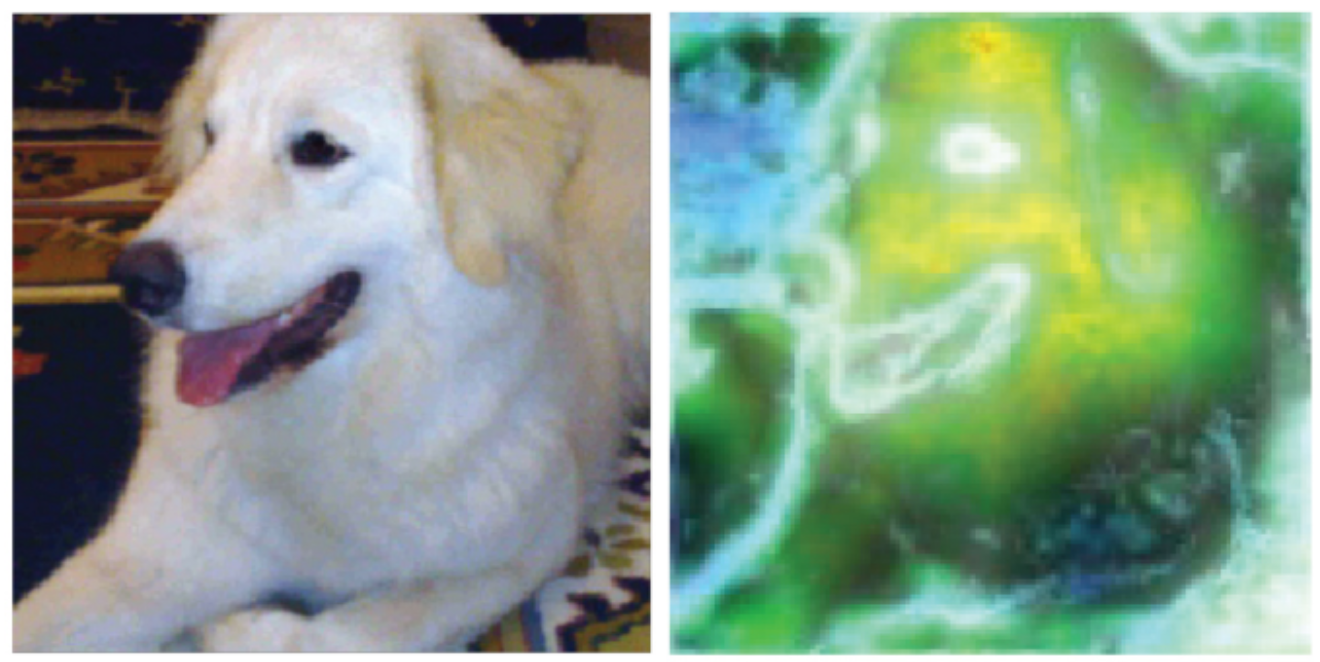
\includegraphics[width = 0.8 \textwidth]{figure/saliencymap}
% \end{figure}
% \end{frame}
%
% \begin{frame}{What is Interpretability?}
% \begin{itemize}
% %\itemsep1em
% \item There is no scientific consensus on the definition of interpretability.
% \item We need to differentiate between interpretations of a model or reality. The latter is distorted by all modeling fallacies involved in predictive modeling, e.g., data quality, under- and overfitting, or model extrapolations.
% \item We use a practical definition of interpretability.
% Think back to the foundations of statistical modeling:  the linear regression model (LM). The LM, with its known equation of beta coefficients, represents a paradigm for statistical interpretability.
% \item It follows that it would be beneficial to create techniques that give us an interpretation similar to the one of an LM.
%
% \end{itemize}
% \end{frame}

% \begin{frame}{Dimensions of Interpretability}

% Interpretation methods can be organized in different dimensions, e.g.:
% \medskip
\begin{framev}[align=top]{Intrinsic, Model-specific, Model-agnostic}
\begin{center}
\resizebox{9.5cm}{3.5cm}{%
\begin{tikzpicture}[every path/.style={->,line width=0.35mm,thick},
every label/.append style={align=left, font=\footnotesize, text width=4cm}]
\node[main node] (1) { Model Interpretation };
\only<1>{\node[main node, fill=lightgray] (2) [below left = 1cm and 0cm of 1]  { Interpretable Models };}
\only<2->{\node[main node] (2) [below left = 1cm and 0cm of 1]  { Interpretable Models };}
\node[main node] (3) [below right = 1cm and -0cm of 1] { Black Box Models };
\only<1,3->{\node[main node] (4) [below left = 1cm and -1cm of 3] { Model-specific Methods  };}
\only<2>{\node[main node, fill=lightgray] (4) [below left = 1cm and -1cm of 3] { Model-specific Methods  };}
\only<-2>{\node[main node] (5) [below right = 1cm and -1cm of 3] { Model-agnostic Methods };}
\only<3->{\node[main node, fill=lightgray] (5) [below right = 1cm and -1cm of 3] { Model-agnostic Methods };}
\draw (1) -- (2);
\draw (1) -- (3);
\draw (3) -- (4);
\draw (3) -- (5);
\end{tikzpicture}}
\end{center}
\only<1>{%
\splitVTT[0.79]{%
\textbf{Intrinsically Interpretable Models:}\\
\spacer[0.25]
\begin{itemizeM}
\item Simple model structure (e.g., weighted sum or tree)
\item Examples: GLMs, decision trees
\item Pro: Additional IML methods not necessarily required
\item Con: \\ Limited model complexity can reduce performance, \\ can still be hard to interpret (many features/interactions)
\end{itemizeM}
}{%
\spacer[0.25]
\begin{center}
\resizebox{2.75cm}{3cm}{%
\begin{tikzpicture}[scale=0.7, transform shape]
\usetikzlibrary{arrows}
\usetikzlibrary{shapes}
\tikzset{treenode/.style={draw, circle, font=\small}}
\tikzset{line/.style={draw, thick}}
\node [treenode, draw=red] (a0) {$a_0$};
\node [treenode, below=0.75cm of a0, xshift=-1cm]  (a1) {$a_1$};
\node [treenode, draw=red, below=0.75cm of a0, xshift=1cm]  (a2) {$a_2$};
\node [treenode, draw=red, below=0.75cm of a2, xshift=-1cm] (a3) {$a_3$};
\node [treenode, below=0.75cm of a2, xshift=1cm]  (a4) {$a_4$};
\node [treenode, below=0.75cm of a3, xshift=-1cm] (a5) {$a_5$};
\node [treenode, below=0.75cm of a3, xshift=1cm]  (a6) {$a_6$};
\path [line] (a0.south) -- + (0,-0.4cm) -| (a1.north) node [midway, above] {$x_1<0.3$};
\path [line] (a0.south) -- +(0,-0.4cm) -|  (a2.north) node [midway, above] {$x_1\geq0.3$};
\path [line] (a2.south) -- + (0,-0.4cm) -| (a3.north) node [midway, above] {$x_1<0.6$};
\path [line] (a2.south) -- +(0,-0.4cm) -|  (a4.north) node [midway, above] {$x_1\geq0.6$};
\path [line] (a3.south) -- + (0,-0.4cm) -| (a5.north) node [midway, above] {$x_2<0.2$};
\path [line] (a3.south) -- +(0,-0.4cm) -|  (a6.north) node [midway, above] {$x_2\geq0.2$};
\end{tikzpicture}}
\end{center}
}}
\only<2>{%
\splitVTT[0.7]{%
\textbf{Model-specific Methods:}\\
\spacer[0.25]
\begin{itemizeM}
\item Designed for specific model types (e.g., NNs)
\item Examples: \\ Gini importance of tree-based models,\\
Layer-wise relevance propagation (LRP)
\item Pro: Exploit model structure
\item Con: Restricted to specific model class
\end{itemizeM}
}{%
\spacer[0.25]
\imageC{figure/catLRP.jpg}
}}
\only<3>{%
\splitVTT[0.7]{%
\textbf{Model-agnostic Methods:}\\
\spacer[0.25]
\begin{itemizeM}
\item In ML: Tune over many model classes \\
$\leadsto$ Unknown which model is best / deployed \\
$\leadsto$ Need for IML methods that work for any model
\item Applied after training (post-hoc)
\item Applicable to intrinsically interpretable models\\
$\leadsto$ provides insights into explanations
\end{itemizeM}
}{%
\spacer[0.25]
\imageC{figure/model_agnostic.jpg}
}}

\end{framev}


\begin{framev}[align=top]{Types of Explanations}
\begin{center}
\begin{tikzpicture}[every path/.style={->,line width=0.35mm,thick},
every label/.append style={align=left, font=\footnotesize, text width=4cm},
scale=0.7, transform shape]
\node[main node] (1) { Model Interpretation };
\only<-4>{\node[main node, fill=lightgray] (2) [below left = 1.3cm and 1.5cm of 1]  { Feature-based Explanations };}
\only<5->{\node[main node] (2) [below left = 1.3cm and 1.5cm of 1]  { Feature-based Explanations };}
\only<1,2,3,4,7,8>{\node[main node, text width=3cm, align=center] (3) [below = 1.3cm of 1] { Data Attribution };}
\only<5,6>{\node[main node, fill=lightgray, text width=3cm, align=center] (3) [below = 1.3cm of 1] { Data Attribution };}
\only<-7>{\node[main node] (4) [below right = 1.3cm and 1.5cm of 1] { Counterfactual Explanations };}
\only<7->{\node[main node, fill=lightgray] (4) [below right = 1.3cm and 1.5cm of 1] { Counterfactual Explanations };}
\draw (1) -- (2);
\draw (1) -- (3);
\draw (1) -- (4);
\end{tikzpicture}
\end{center}
\only<1>{%
\textbf{Feature-based Explanations:}\\
\spacer[0.25]
\begin{itemizeM}
\item Analyze the role of individual features in model behavior.
\item Types of feature-based explanations: \\
\begin{itemizeS}[scriptsize]
\item Feature Importance
\item Feature Effects
\item Feature Interactions
\end{itemizeS}
\item Common principle:
Vary or perturb feature values and observe changes in predictions, variance, or performance.
\end{itemizeM}
}
\only<3>{%
\textbf{Feature Effects} indicate changes (direction and magnitude) in model prediction due to changes in feature values.\\
\spacer[0.25]
\splitVTT[0.4]{%
\begin{itemizeM}
\item Model-agnostic methods: \\ ICE curves, PD plots $\hdots$
\item Pendant in linear models: \\ Weights / coefficients $\theta_j$
\item Further examples:
ALE, SHAP, and LIME
\end{itemizeM}
}{%
\spacer[0.25]
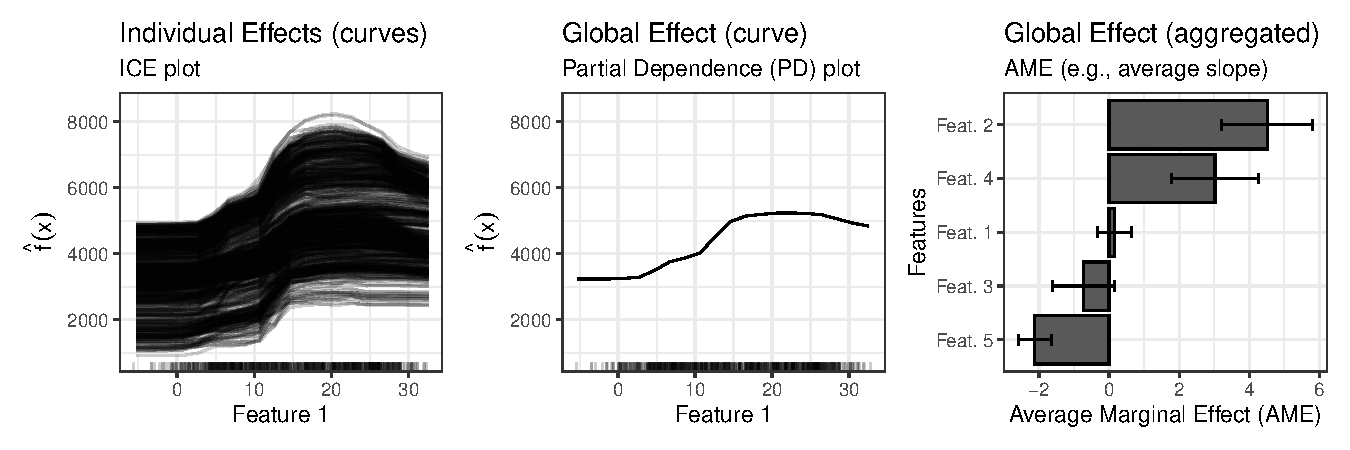
\includegraphics[page=1, width=\textwidth, trim=0 0 215 0, clip]{figure/feature-effect}
}}
\only<2>{%
\textbf{Feature Importance} quantifies relevance of features, e.g., their contribution to model prediction, predictive performance, or prediction variance.\\
\spacer[0.25]
\splitVTT[0.55]{%
\begin{itemizeM}
\item Model-agnostic methods: PFI, $\hdots$
\item Pendant in linear models: t-statistic, p-value (significant effect)
\end{itemizeM}
}{%
\spacer[0.25]
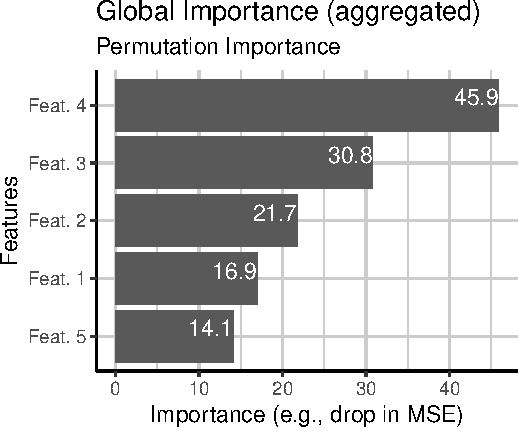
\includegraphics[page=1, width=0.9\textwidth, trim=0 0 0 30, clip]{figure/feature-importance}
}}
\only<4>{%
\splitVTT[0.51]{%
\textbf{Feature Interaction:}\\
How combinations of features jointly affect predictions.
\begin{itemizeM}
\item Model-agnostic methods: \\ Friedman's H-statistic
\item Pendant in linear models: \\ Coefficients of interaction terms $\theta_{jk}$
\end{itemizeM}
}{%
\spacer[0.25]
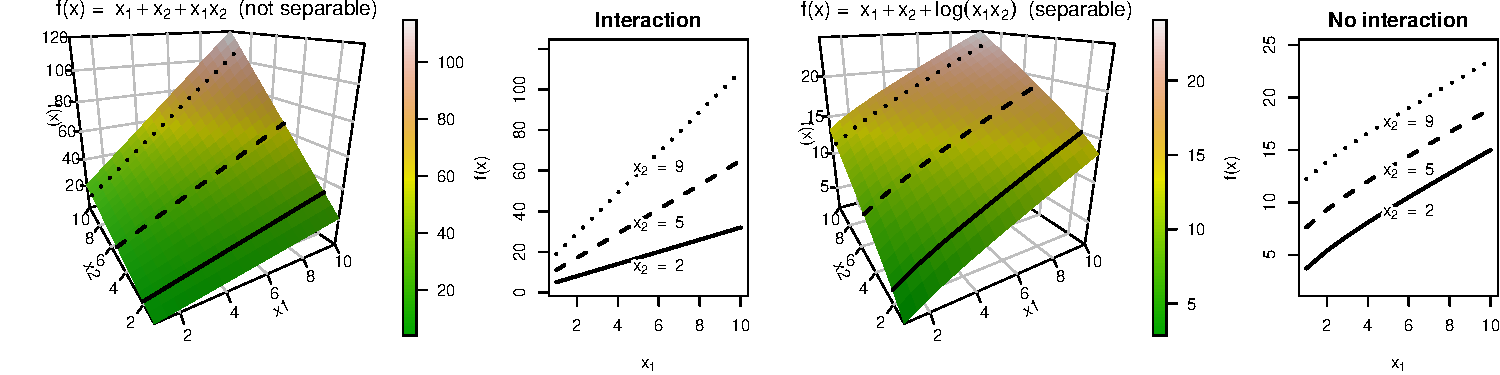
\includegraphics[width=\textwidth, trim={0cm 0cm 12cm 0cm}, clip]{figure/interaction_separable_2}
}}
\only<5-6>{%
\textbf{Data Attribution:} Identify training instances that most influenced a prediction.\\
\spacer[0.25]
\textbf{Example:} A model should distinguish muffins and dogs.\\
\spacer[0.25]
}
\only<5>{%
Question: Why does it misclassify this dog image (test point) as a muffin?
\imageC[0.5]{figure/Chihuahua_or_muffin_model.png}
}
\only<6>{%
\textbf{Approach}: Measure how perturbations to training data affect prediction/loss.\\
\spacer[0.25]
\splitVCC[0.5]{%
\imageC[0.88]{figure/Chihuahua_or_muffin.png}
}{%
\begin{itemizeM}
\item[$\leadsto$] Influential training instances drive prediction of test points.
\item[$\leadsto$] If these resemble muffins, the model may predict muffin instead of dog.
\end{itemizeM}
}}
\only<7>{%
\spacer[0.25]
\splitVCC[0.6]{%
\textbf{Counterfactual Explanations:}\\
\spacer[0.25]
\begin{itemizeM}
\item Identify smallest necessary change in feature values so that a desired outcome is predicted
\item Contrastive explanations
\item Diverse counterfactuals
\item Feasible \& actionable explanations
\end{itemizeM}
}{%
\imageC{figure/counterfactuals_obj}
}}
\only<8>{%
\textbf{Example} (loan application):
\imageC[0.6]{figure/counterfactual.pdf}
}
\end{framev}




% \begin{frame}{Feature Effects vs. Feature Importance}

% 	\textbf{Feature Effects} indicate the change in prediction due to changes in feature values.
% 	\medskip
% 	\begin{center}
% 		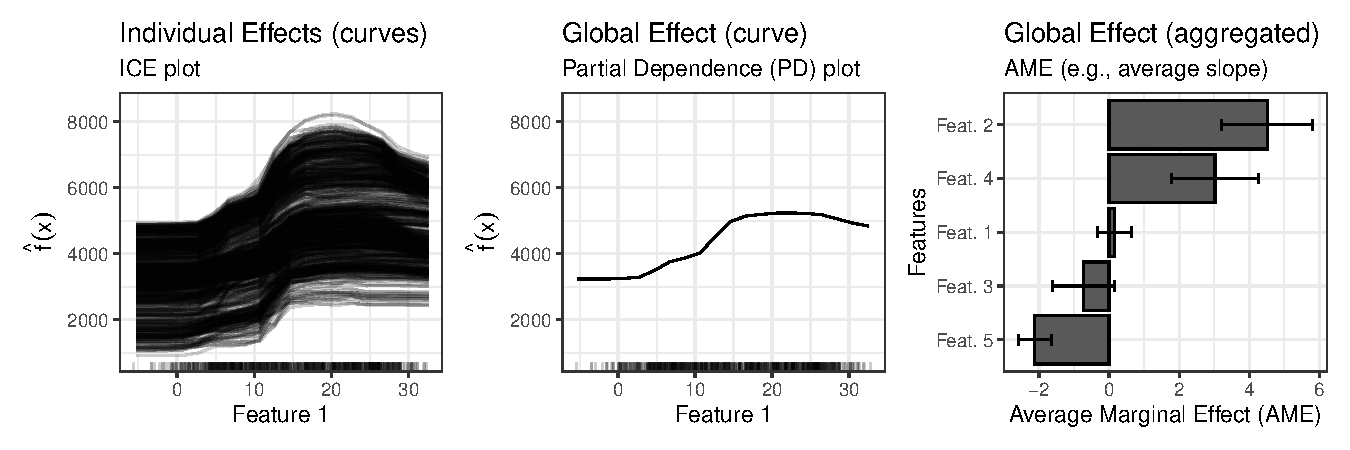
\includegraphics[page=1, width=0.7\textwidth, trim=0 0 215 0, clip]{figure/feature-effect}
% 	\end{center}
% 	\begin{itemize}
% 		\item Model-agnostic methods: ICE curves, PD plots $\hdots$
% 		\item Pendant in linear models: Regression coefficient $\theta_j$
% 	\end{itemize}
% \end{frame}

% \begin{frame}{Feature Effects vs. Feature Importance}

% 	\textbf{Feature importance} methods rank features by how much they contribute to the predictive performance or prediction variance of the model.
% 	\begin{center}
% 		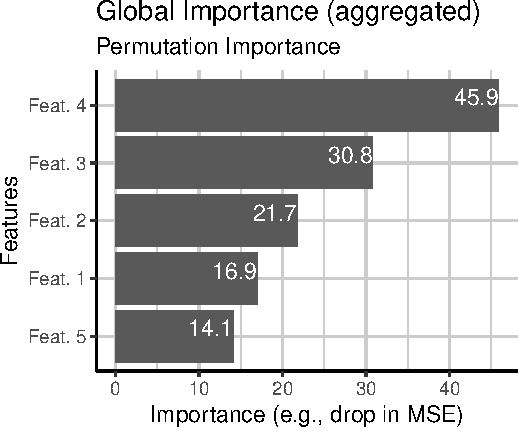
\includegraphics[page=1, width=0.4\textwidth]{figure/feature-importance}
% 	\end{center}
% 	\begin{itemize}
% 		%\itemsep1em
% 		\item Model-agnostic methods: PFI, $\hdots$
% 		\item Pendant in linear models: t-statistic, p-value (significant effect)
% 	\end{itemize}

% \end{frame}


% \begin{frame}{Explanation using training instances~\citebutton{Koh et al. 2017}{https://arxiv.org/pdf/1703.04730.pdf}}

% 	\textbf{Data attribution:} Which training instances results in the decision for the instance $x$ of the model?
% 	\begin{center}
% 		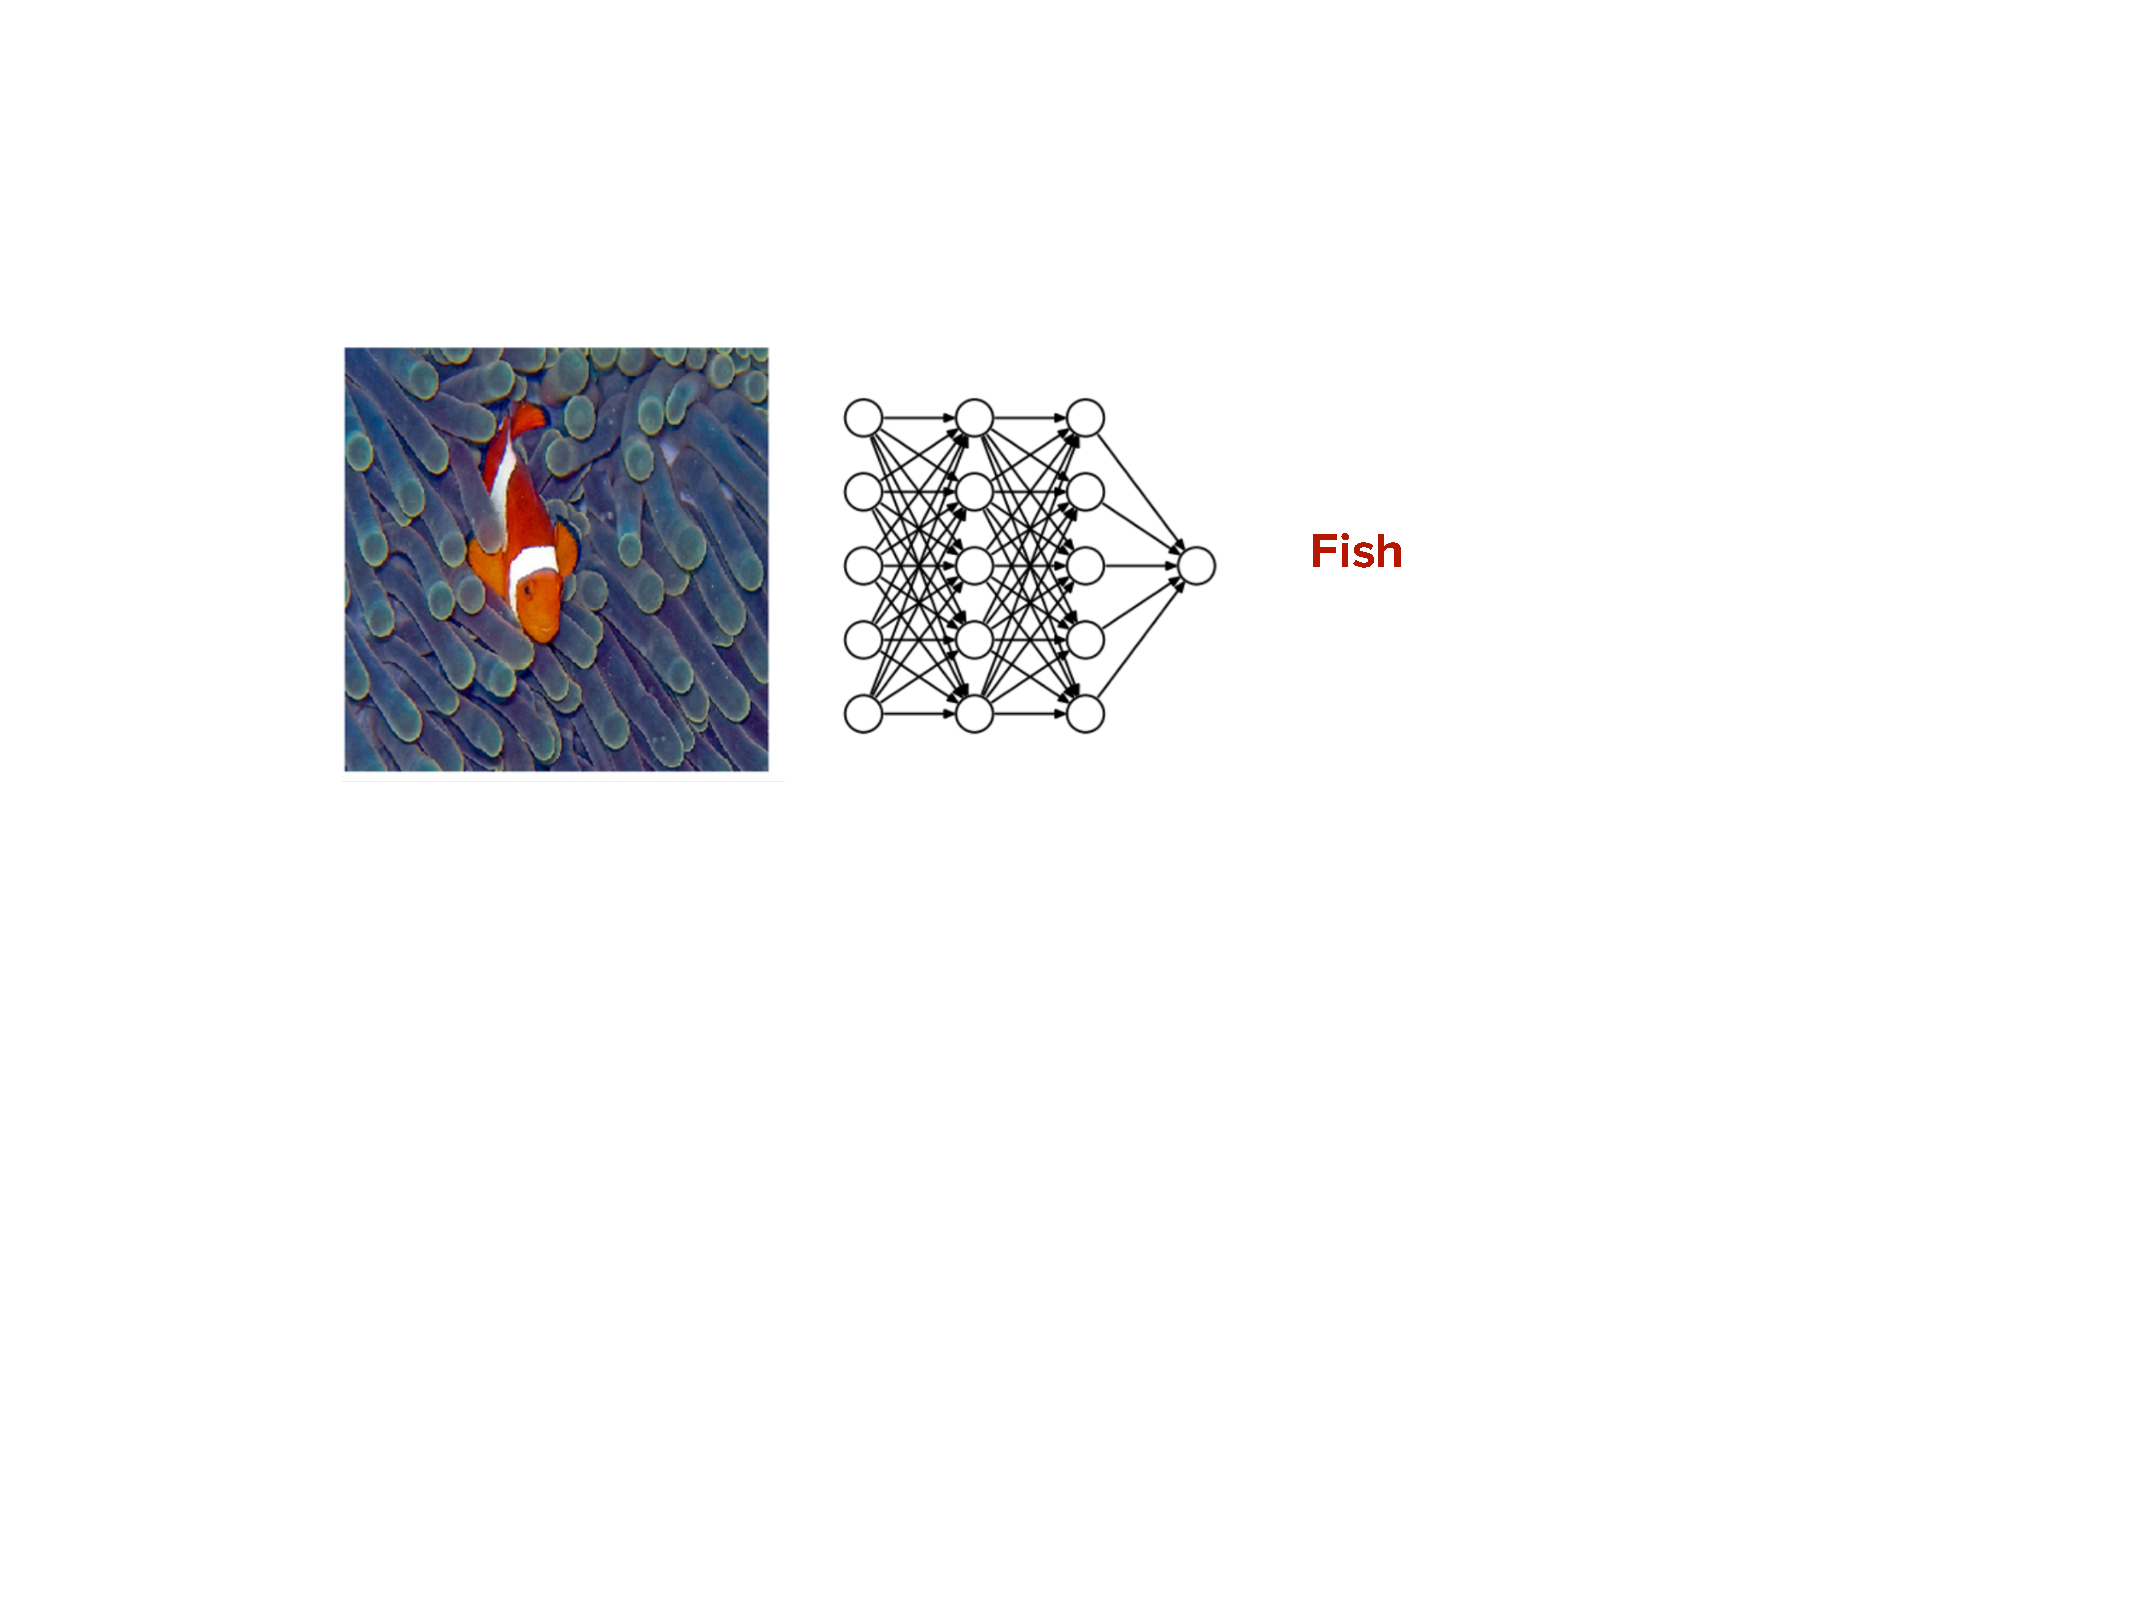
\includegraphics[page=1, width=0.7\textwidth]{figure/fish-attribution.pdf}
% 	\end{center}
% \end{frame}

% \begin{frame}{Explanation using training instances~\citebutton{Koh et al. 2017}{https://arxiv.org/pdf/1703.04730.pdf}}
% 	\textbf{Data attribution:} Which training instances results in the decision for the instance $x$ of the model?
% 	\begin{center}
% 		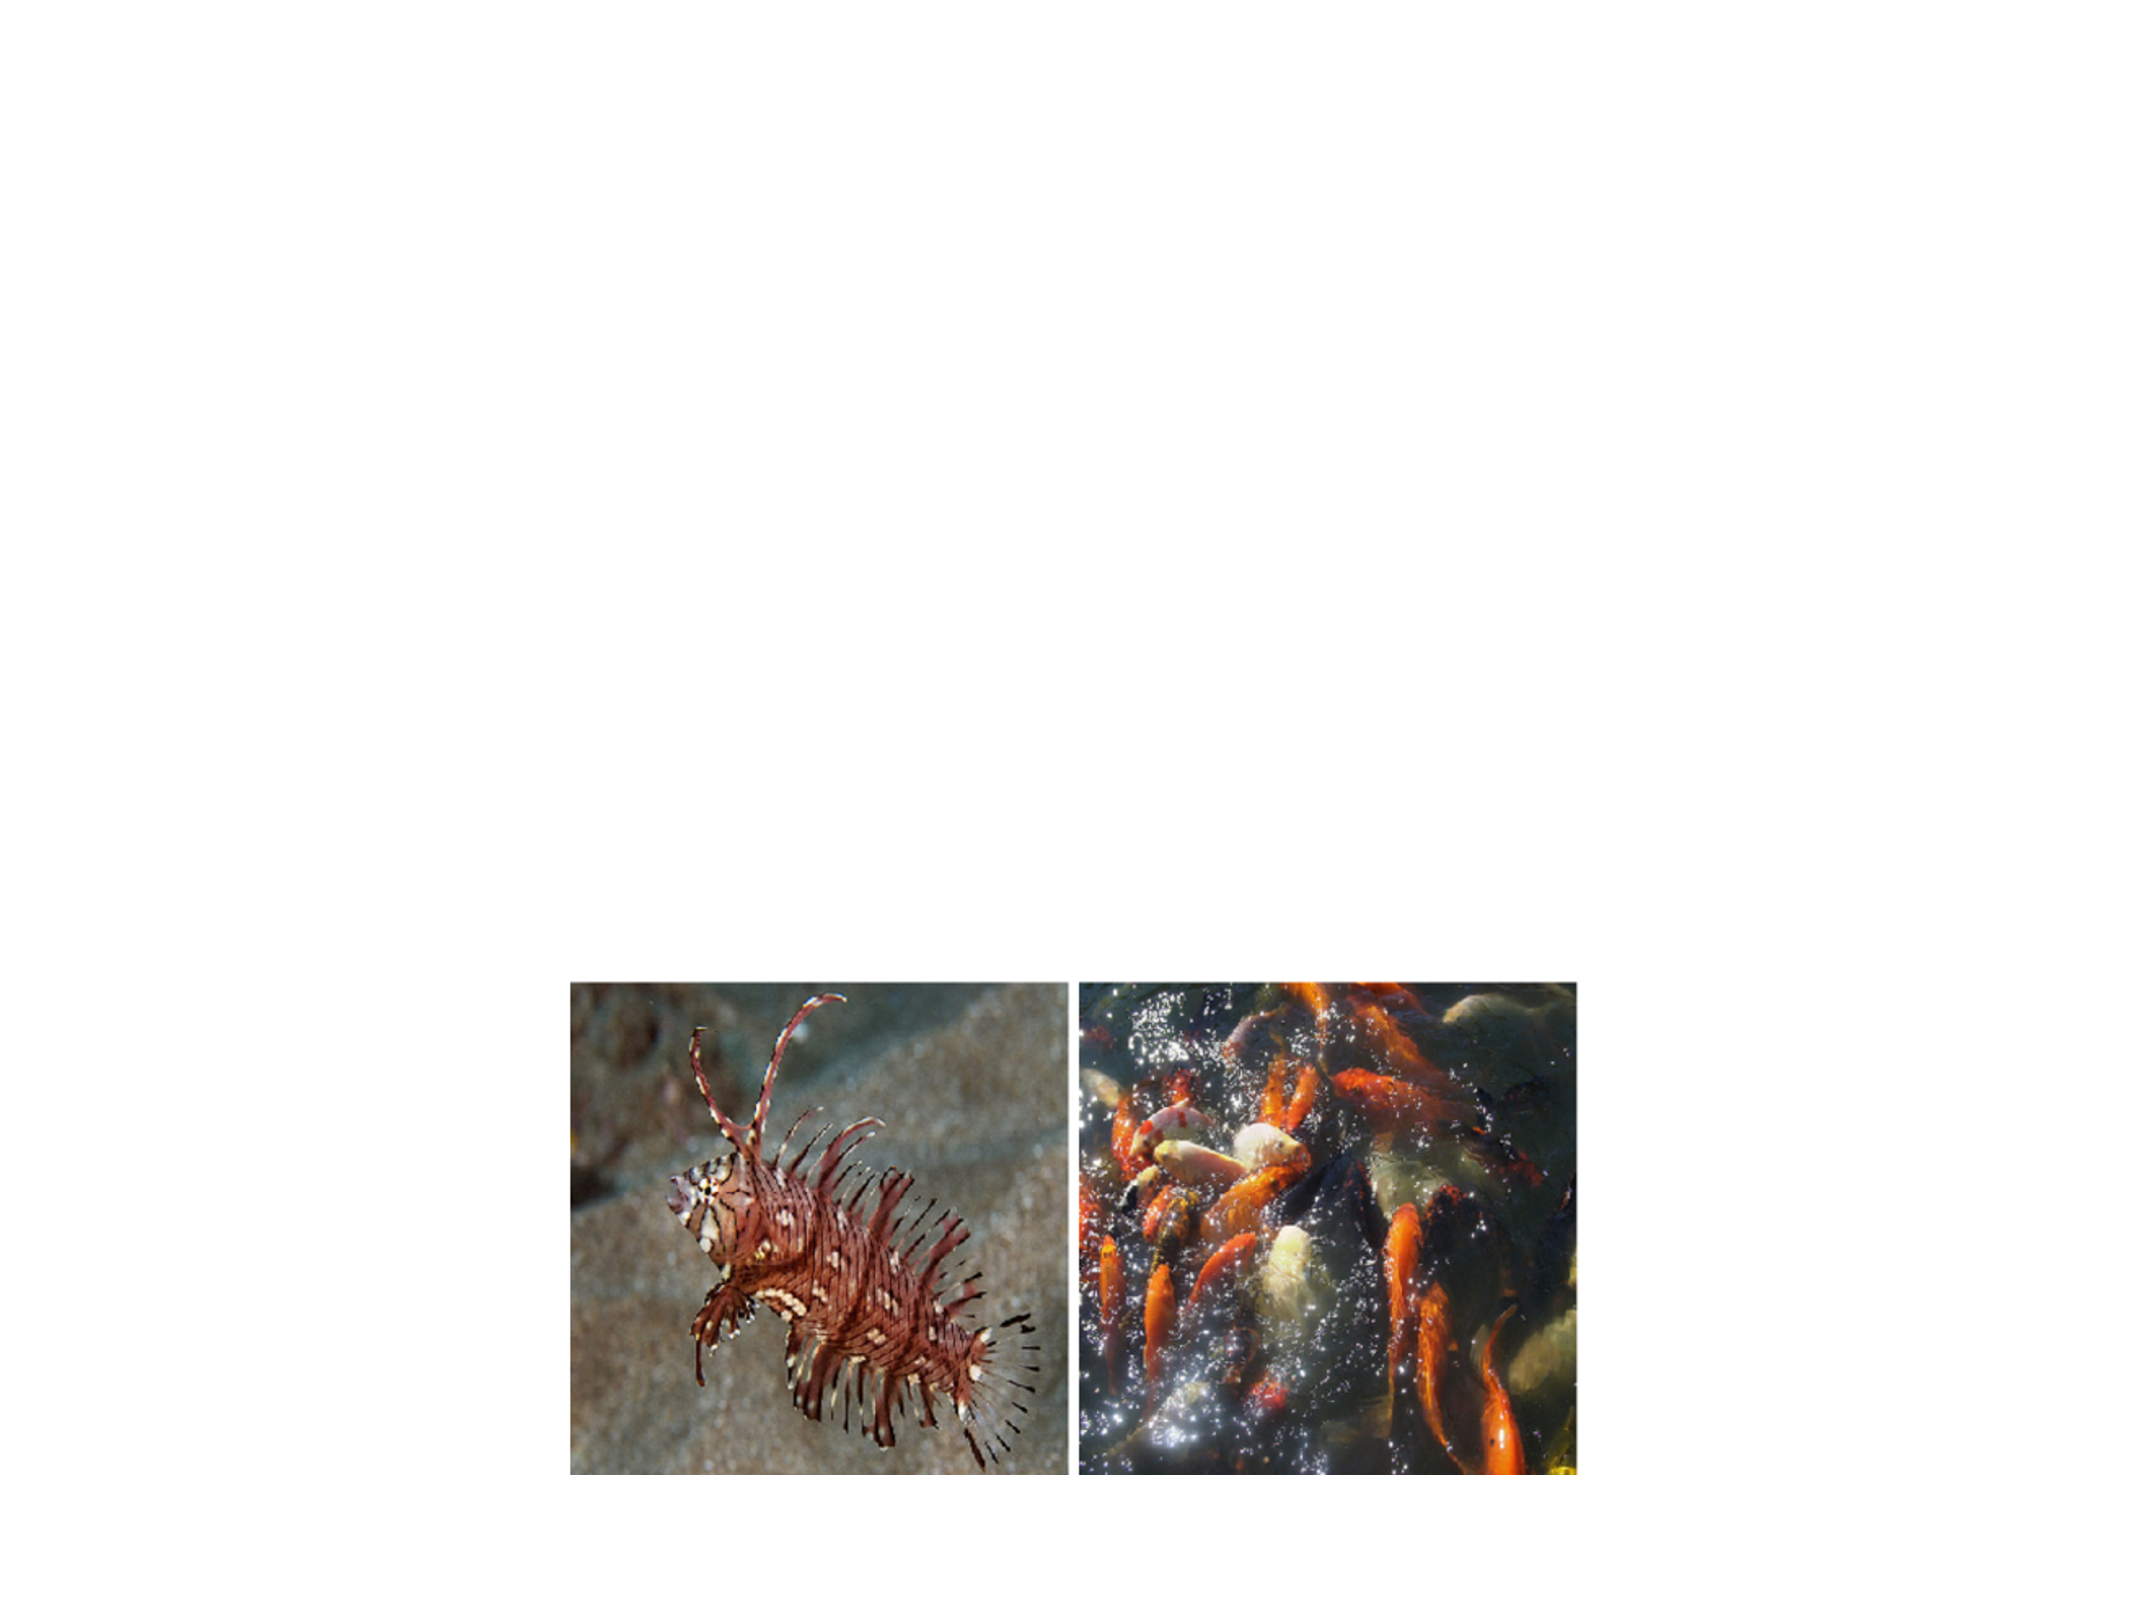
\includegraphics[page=1, width=0.7\textwidth]{figure/prototypes-fish.pdf}
% 	\end{center}
% 	\begin{itemize}
% 		\item Methods:
% 		Influence functions, prototype generation
% 	\end{itemize}
% \end{frame}

% \begin{frame}{Explanation using training instances}
%     \textbf{Data attribution:} Which training instances results in the decision for the instance $x$ of the model?
% 	\vspace{0.4cm}
% 	\begin{center}
% 		
\includegraphics[page=1, width=0.8\textwidth]{figure/Chihuahua_or_muffin_model.png}
% 	\end{center}
% \end{frame}

% \begin{frame}{Explanation using training instances}
% 	\textbf{Data attribution:} Which training instances results in the decision for the instance $x$ of the model?
% 	\begin{center}
% 		
\includegraphics[page=1, width=0.3\textwidth]{figure/Chihuahua_or_muffin.png}
% 	\end{center}
% 	\begin{itemize}
% 		\item[$\leadsto$]  Model chose the wrong output
% 	\end{itemize}
% \end{frame}

% \begin{frame}{Explanation using Counterfactuals}
%     A counterfactual is small ``imperceptible'' change in $x$ causing a different prediction.\\
%     $\leadsto$ What if a small difference $ |x - x'| \leq \epsilon$ to $x$ causes a large change in the model output ?

%     \textbf{Example} (loan application):
% 	\begin{center}
% 	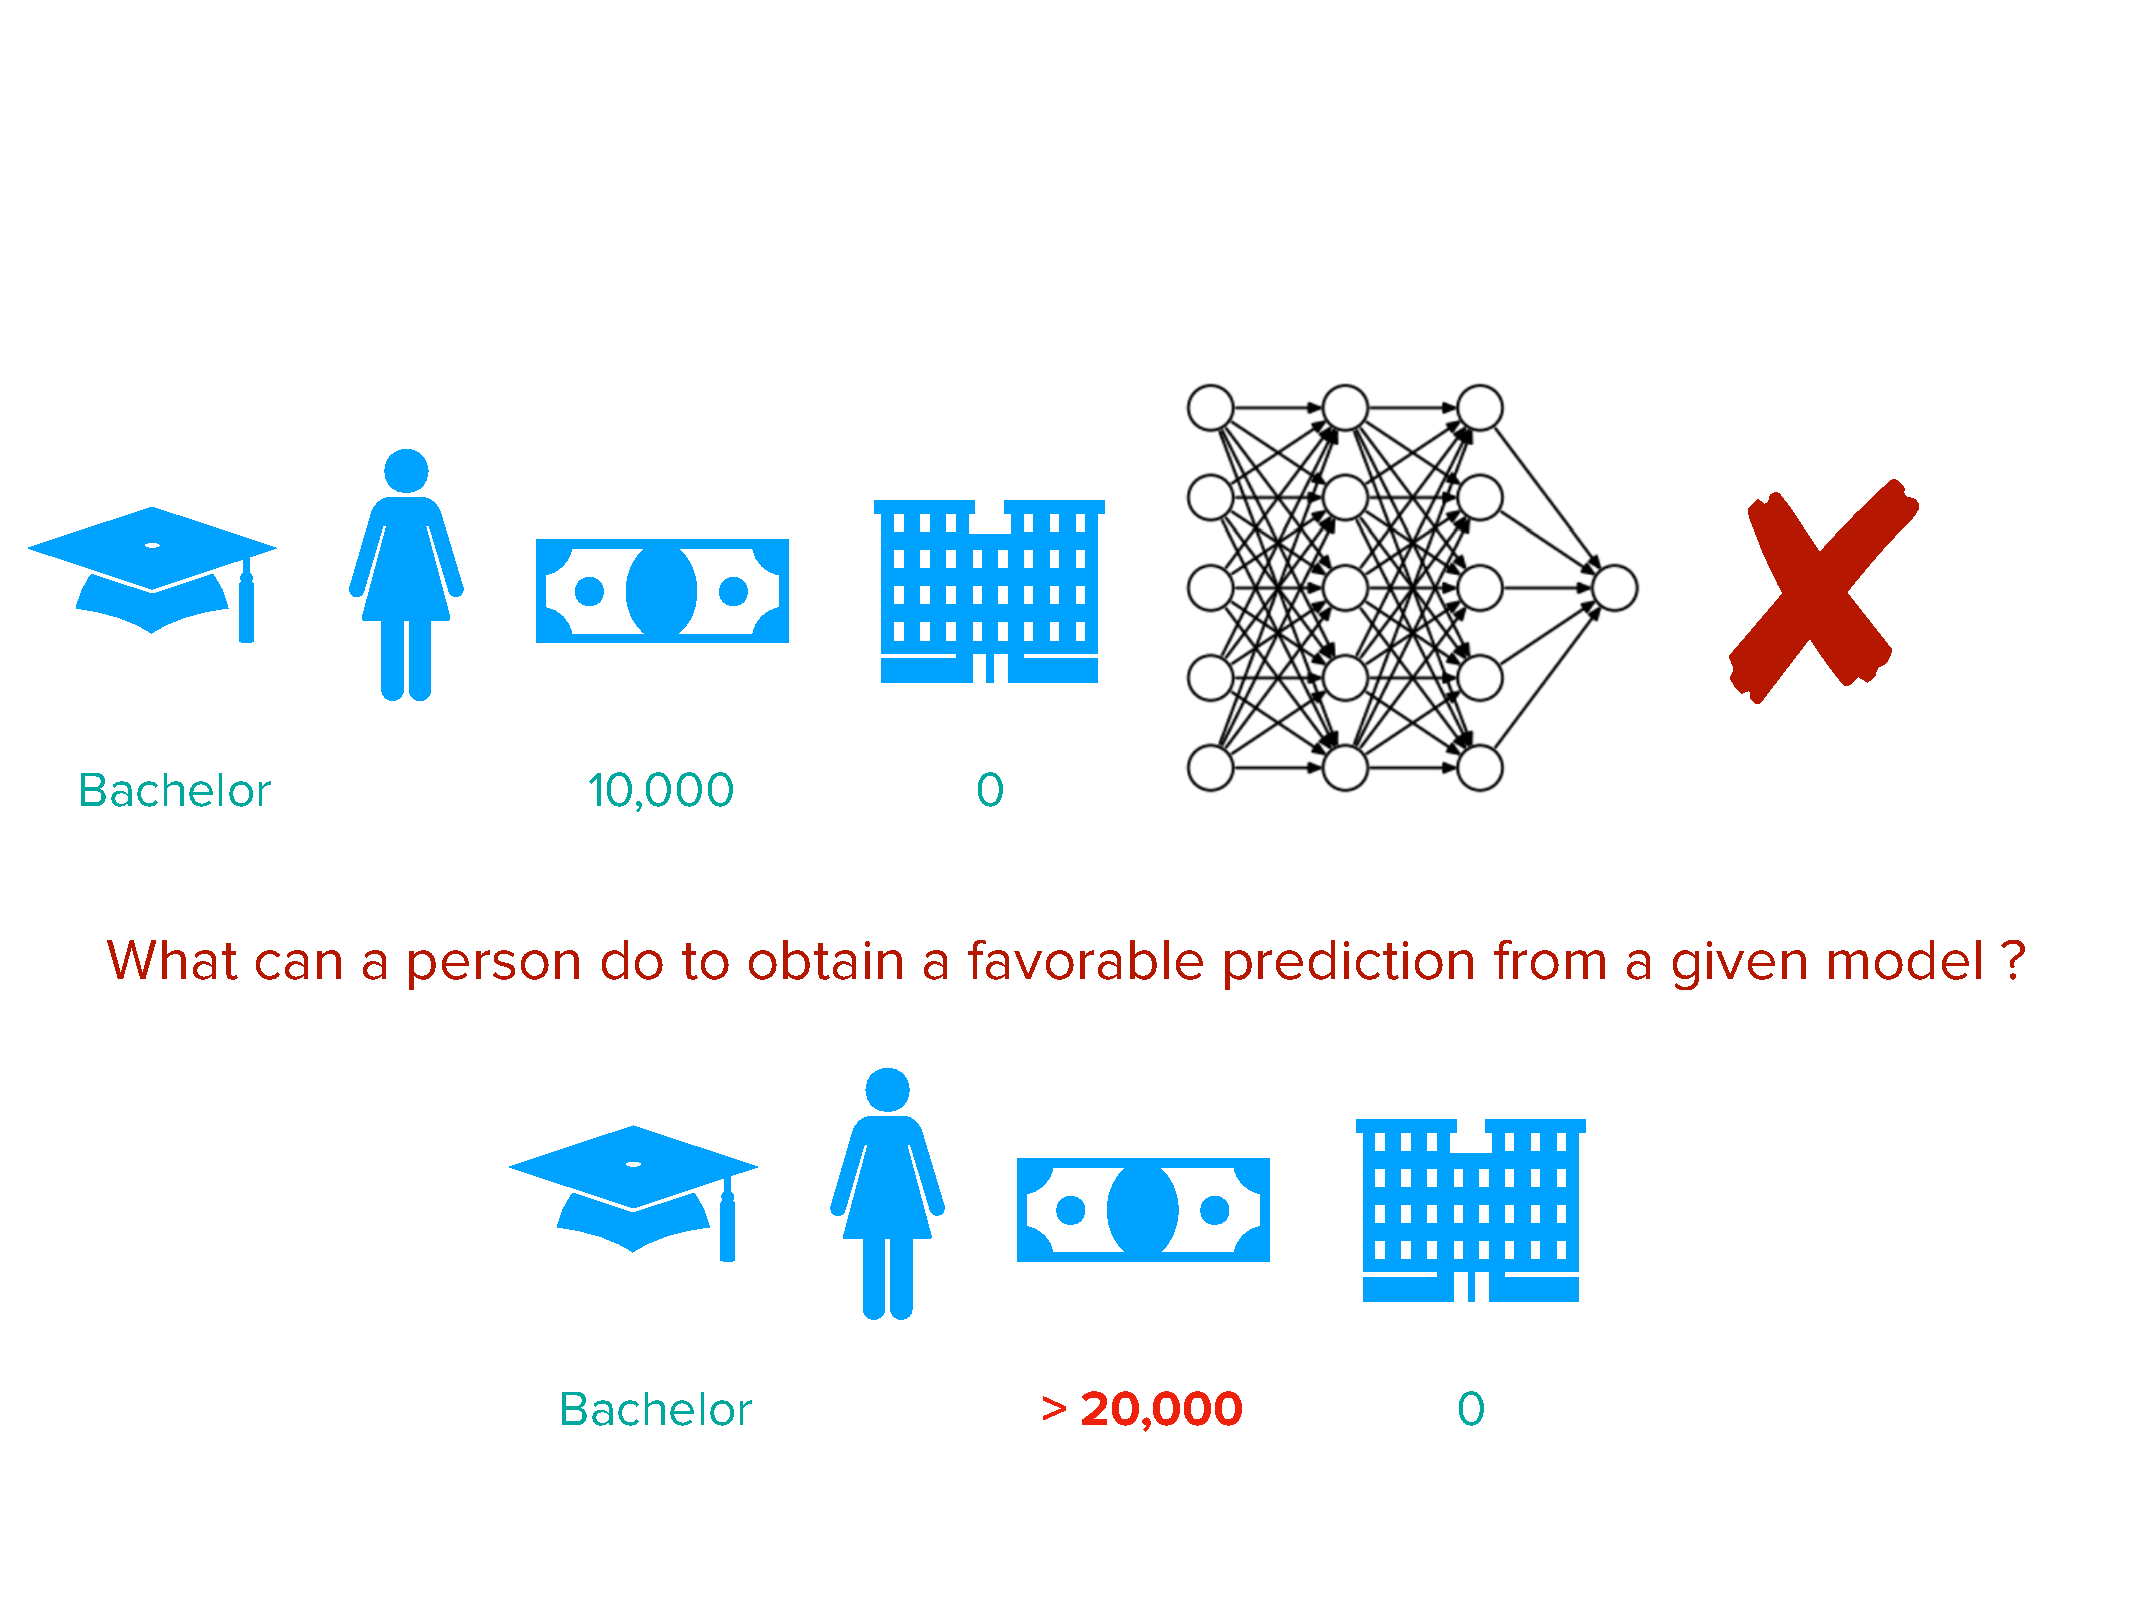
\includegraphics[page=1, width=0.7\textwidth]{figure/counterfactual.pdf}
% 	\end{center}

% \end{frame}

\begin{framev}[align=top]{Local, Global, and Regional Explanations}
\splitVTT[0.75]{%
\only<1->{%
\textbf{Local:} Explain model behavior for \textbf{single instances}:
\begin{itemizeM}
\item Provide nuanced instance-specific insights
\item Crucial for complex models where features typically affect instances differently (due to interactions)
\item Examples: Counterfactuals, LIME, SHAP, ICE
\end{itemizeM}
}
\only<2->{%
\textbf{Global:} Explain model behavior for \textbf{entire input space}:
\begin{itemizeM}
\item Provide high-level insights into model behavior, \\ often by aggregating local explanations
\item Easier to communicate but loss of detail \& over-simplification (hides differences)
\item Examples: PD plots, ALE plots, PFI
\end{itemizeM}
}
\only<3->{%
\textbf{Regional explanations} -- for \textbf{subspaces} / \textbf{regions}:
\begin{itemizeM}
\item Compromise between nuanced \& high-level insights
\item Useful when local explanations group well without losing much detail
\end{itemizeM}
}
}{%
\spacer[0.25]
\imageC[0.95]{figure/local_regional_global_col.png}
}
\end{framev}


% -------------------------------------------------
% Local – Global – Regional explanations (Bike-sharing)
% -------------------------------------------------
\begin{framev}[align=top]{Local, Global, Regional Explanations}
\splitVTT[0.6]{%
\begin{itemizeM}
\item<1-> \textbf{Local} (red): ICE curves for one instance\\
$\leadsto$ Detailed but cluttered/obscure pattern
\item<1-> \textbf{Global} (blue): PDP averaged over \emph{all} days\\
$\leadsto$ Averaged curve hides heterogeneity
\item<2-> \textbf{Regional}: Split data on \texttt{workingday}\\
$\leadsto$ Preserves detail without overload\\
$\leadsto$ Challenge: find regions automatically
\end{itemizeM}
}{%
\spacer[0.25]
\includegraphics<1->[trim=0 0 0 20, clip, width=\textwidth]{figure/01_bike_sharing_dataset_18_1.png}
}
\only<2->{%
\twobytwo{
\spacer[0.25]
\centering \scriptsize Region 1 (working day): morning and evening peak
}{
\spacer[0.25]
\centering \scriptsize Region 2 (non-working day): late-morning leisure peak
}{
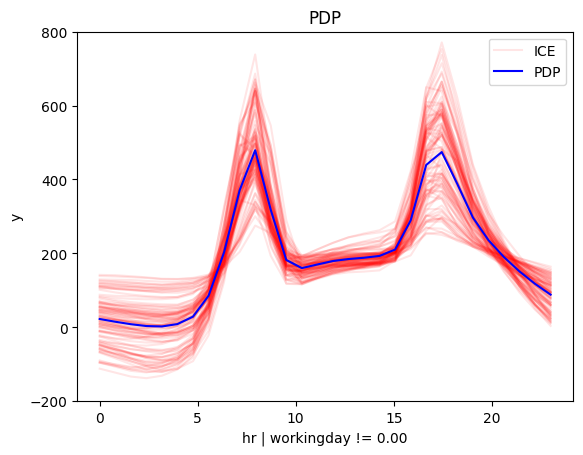
\includegraphics[trim=0 0 0 20, clip, width=0.99\textwidth]{figure/01_bike_sharing_dataset_28_1.png}
}{
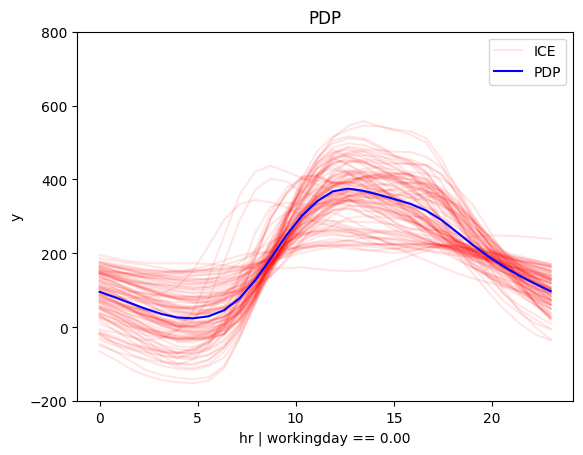
\includegraphics[trim=0 0 0 20, clip, width=0.99\textwidth]{figure/01_bike_sharing_dataset_28_0.png}
}}
\end{framev}



\begin{framev}[align=top]{Fixed Model vs. Refits}
\begin{itemizeM}
\item Global interpretation methods: Input: model $+$ data, output: explanations\\
$\leadsto$ Explanations can be viewed as statistical estimators
\item[] \imageC[0.9]{figure/fixed_model_vs_refits.jpg}
\item Situation in ML: Deployed model is trained on all available data\\
$\leadsto$ No unseen test data left to, e.g., reliably estimate performance\\
$\leadsto$ IML method could use same data model was trained on \\
$\leadsto$ But: Some IML methods require measuring loss on unseen test data
\item Alternative: Explain the inducer that created the model (not a fixed model)\\
$\leadsto$ Idea: Use resample strategies (e.g. CV) as in performance estimation\\
$\leadsto$ Requires refitting
\end{itemizeM}
\end{framev}

\begin{framev}[align=top]{Levels of interpretability}
\begin{center}
\spacer[-0.5]
\begin{tabular}{
>{\centering\arraybackslash}m{0.08\textwidth} >{\centering\arraybackslash}m{0.001\textwidth} >{\centering\arraybackslash}m{0.38\textwidth} >{\centering\arraybackslash}m{0.001\textwidth} >{\centering\arraybackslash}m{0.38\textwidth}}
&& \textbf{Research question} && \textbf{Objects of analysis} \\ &&&\\[-2ex]
1\textsuperscript{st} level view && \cellcolor{imldarkblue}\color{white}How to explain a given model fitted on a data set? && \cellcolor{imldarkblue}\color{white} (deployed) model \centerline{$\theta \mapsto \hat{f}(\theta)$} \leavevmode\\
\only<2->{&&&\\[-1.5ex] 2\textsuperscript{nd} level view && \cellcolor{imlmedblue}\color{white}How does an optimizer choose a model based on a data set? && \cellcolor{imlmedblue}\color{white} Model selection process (e.g., decisions made by AutoML systems or HPO) \leavevmode\\}
\only<3>{&&&\\[-1.5ex] 3\textsuperscript{rd} level view && \cellcolor{imllightblue}\color{white}How do data properties relate to performance of a learner and its hyperparameters? && \cellcolor{imllightblue}\color{white} Properties of ML algorithms in general (benchmark) \leavevmode\\}
\end{tabular}
\only<1>{\spacer[0.3]}
\includegraphics<1>[page=1, width=0.8\textwidth]{figure/blackbox levels.pdf}
\only<2>{\spacer[-0.3]}
\includegraphics<2>[page=2, width=0.8\textwidth]{figure/blackbox levels.pdf}
\only<3>{\spacer[0.05]}
\includegraphics<3>[page=3, width=0.8\textwidth]{figure/blackbox levels.pdf}
\end{center}
\end{framev}

\endlecture
\end{document}


%%
